\chapter{Methodology}

\AddToShipoutPictureBG*{%
  \AtPageUpperLeft{%
    \hspace*{18.25cm}%
    \raisebox{-3cm}{%
      \makebox[0pt][r]{\parbox{\textwidth}{\begin{flushright}\textit{``Premature optimization is the root of all evil.''}\\
      Donald Knuth\end{flushright}}}
}}}%

The measurement uncertainty has been taken into account, but not the simulation uncertainty. The objectives of this chapter are to create a pool of candidate inputs with associated uncertainties, select the sensitivity analysis method to identify key system parameters, and develop the model calibration algorithm to auto-capture the system dynamics.

\section{Overview}

Model calibration is commonly regarded as an inverse estimation process where the selected input parameters are tuned to reconcile the outputs from simulation as closely as possible to the measurements. Generally there are three technical parts: model pre-establishment, model calibration, and model post-evaluation. In this study, the UWG is selected as the simulation engine to implement the calibration, since it can be applied to different climate zones and urban configurations to yield an estimation of the UHI effect to some extent.

\begin{figure}
\centering
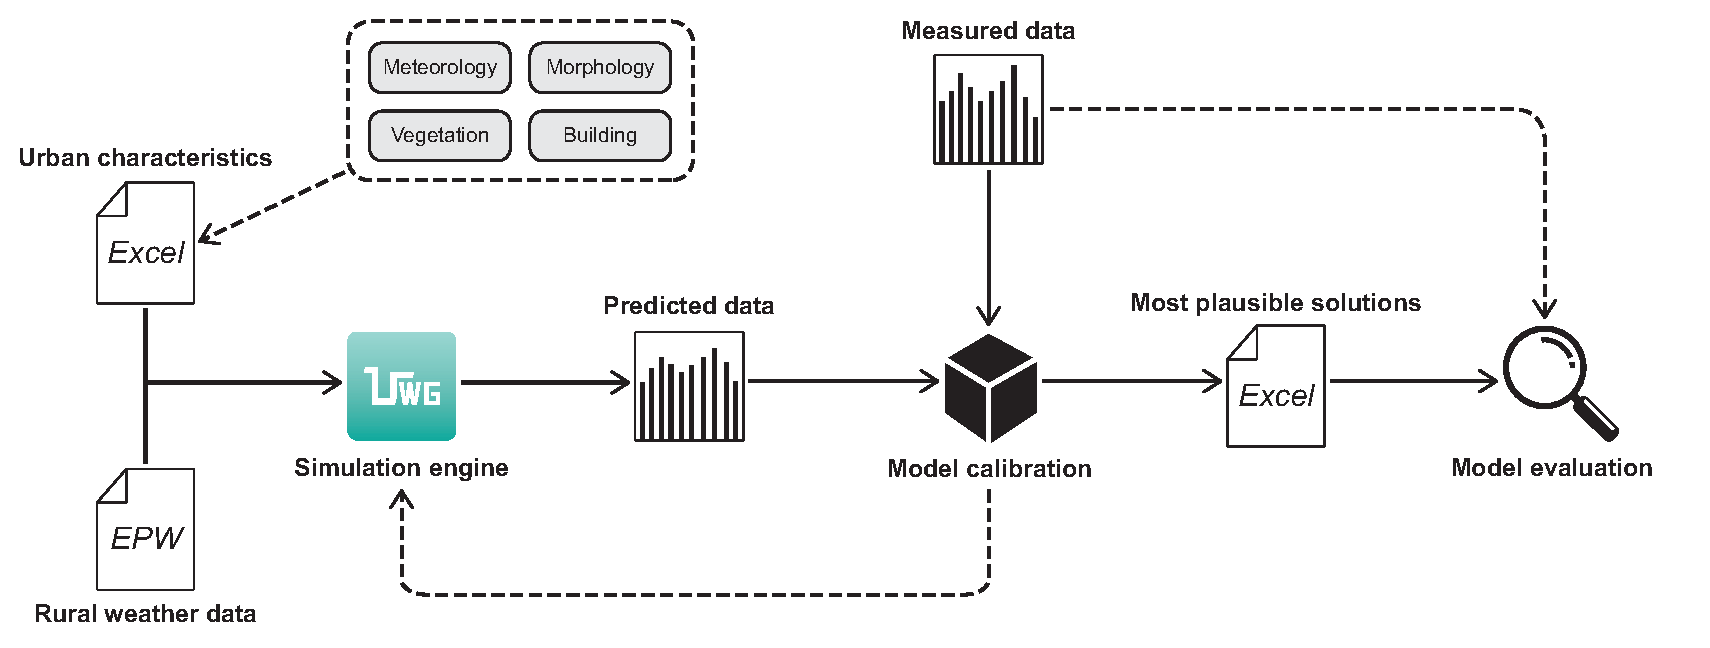
\includegraphics[width=.95\linewidth,trim=0 0 10 0,clip]{Figure4-1.eps}
\caption{General workflow of model calibration via the UWG.}
\end{figure}

As shown in \textbf{Figure 4-1}, the whole process starts by establishing case-specific UWG input files via the Excel interface facilitated by \textsc{Matlab}. Then, the simulated outputs are collected along with the measured data to initiate the calibration algorithm. Once the most plausible solutions are produced, they will be further examined to evaluate the system behavior.

The core methodology of calibrating a simulation program against the real data needs to be rational, robust, and efficient. Besides, it should have the flexibility for different users with different levels of preference and target. It is recognized from previous studies \cite{saltelli2002sensitivity,oliva2003model} that calibrating a detailed model with numerous parameters is a highly underdetermined problem, which may yield multiple non-unique solutions. The conventional wisdom is that once a model is calibrated in a certain sense, the effect of some intended adaption measures (i.e., parameter variations) could be assessed with a high level of confidence. This idea could be misleading since the urban microclimate condition is the aggregate behavior of many components in the system. Even if the optimization algorithm exhibits an overall good calibration performance, some of the individual parameters might be inaccurately identified. Therefore, it is unlikely that any one optimal solution can be deemed the ``best.'' Instead, we posit that it is more reasonable to identify the most plausible solutions (that are able to perform well under some specified measure) with associated uncertainties for a fairly robust calibration method.

Within this context, the calibration framework developed in this thesis generally enjoys the methodology proposed by Reddy et al. \cite{sun2006calibration,reddy2007calibrating}. The basic structure, shown in \textbf{Figure 4-2}, involves the following five steps:

\begin{figure}[h]
\centering
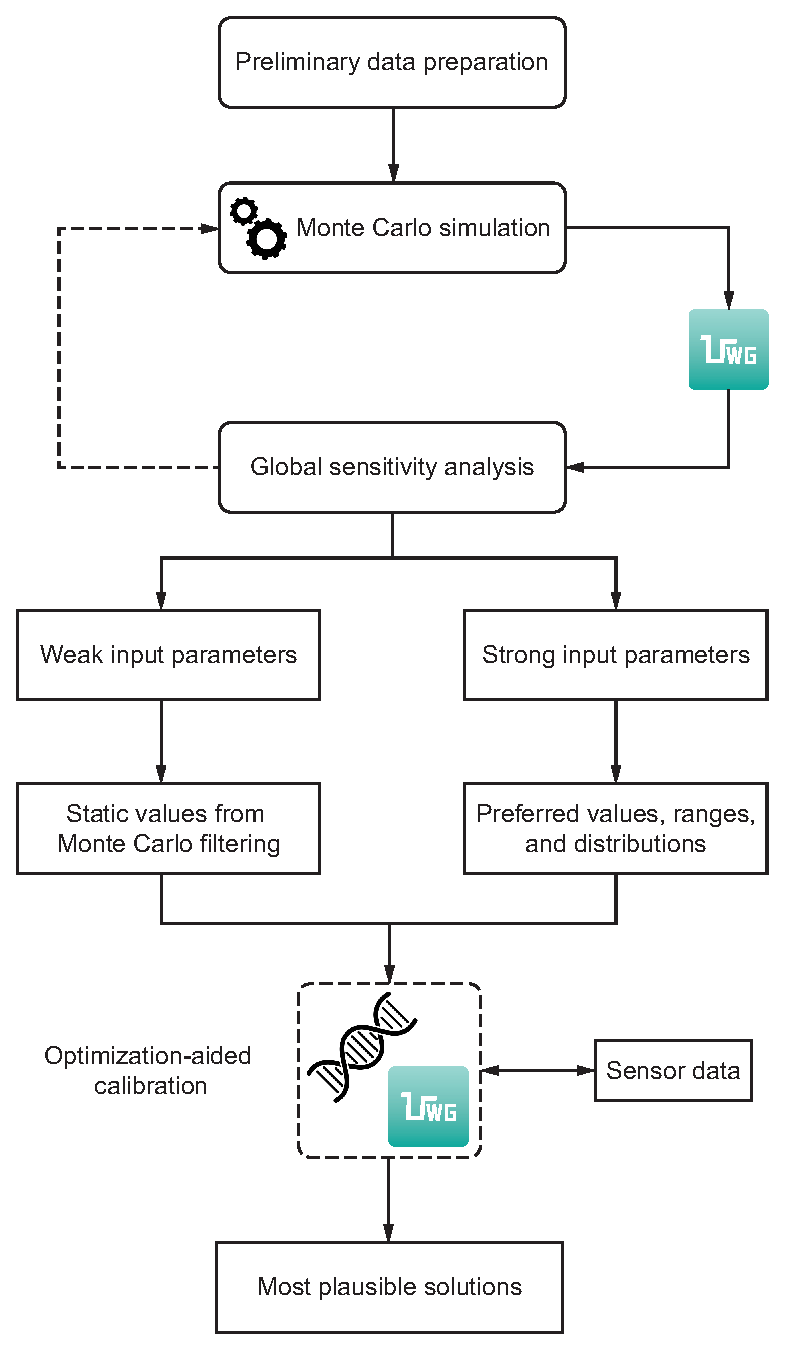
\includegraphics[width=.53\linewidth]{Figure4-2.eps}
\caption{Structure of an optimization-aided calibration method via the UWG.}
\end{figure}

\begin{enumerate}[\textit{Step} \itshape1:]
  \item Prepare the baseline information of the neighborhood area as precisely as possible. This enables the UWG to simulate the microclimate condition in the target street-level area.
  \item Identify a set of candidate parameters along with their preferred defaults and ranges. This provides some potential options for model calibration and adaption measures.
  \item Perform uncertainty and sensitivity analysis with different combinations of the inputs. This improves the understanding of the system by identifying the significant parameters.
  \item Apply guided search and optimization algorithm to refine the solutions automatically. This results in a set of plausible solutions that may represent the system dynamics.
  \item Evaluate the calibration effectiveness and efficiency of these solutions under uncertainty. This examines how likely the calibrated model is to yield biased system predictions.
\end{enumerate}

Since \textbf{Chapter 3} has detailed the baseline model of the present case study (\textit{Step 1}), the following subsections will further illustrate the technical guidelines and procedures of sensitivity/uncertainty analysis and model calibration (\textit{Steps 2-4}).

\section{Candidate input parameter}

Before conducting sensitivity/uncertainty analysis and model calibration, it is important to determine what input parameters with corresponding uncertainties are to be studied and what method is to be used. 

Defining a pool of candidate input parameters with reasonable uncertainties is often an arduous task which requires a sensible engineering judgment. Based on previous studies \cite{bueno2013urban,bueno2014computationally,bueno2013calculation} and local engineering practices \cite{martin2015estimation,deru2011us,radhi2009evaluating,afshari2014life}, 30 parameters are selected and categorized into four groups for the present study (see \textbf{Table 4.1}). For the parameters in the group of meteorological factors, urban characteristics, and vegetation variables, the uncertainty ranges are intentionally defined rather broadly in order to take all the possible uncertainties into account. In terms of most building-related parameters for a specific case study, values could be obtained within relatively small uncertainty ranges from available reports and technical specifications. The corresponding values of the remaining unselected parameters are taken as defaults from the data shown in \textbf{Tables 3.1 and 3.3}. Yet, disregarding uncertain input parameters can cause a fraction of the total output uncertainty to remain unexplained in the results, which should be considered in the interpretation of the outcomes.

Uncertainty can be generally classified as \textit{aleatory} and \textit{epistemic} uncertainty \cite{helton1996guest}. Aleatory uncertainty refers to the inherent randomness in the system behavior, while epistemic uncertainty comes from a lack of knowledge about the appropriate value in a specific application. The parameters associated with aleatory uncertainty are assumed to have a \textit{normal} distribution, which is suitable for measured physical properties. On the other hand, the parameters associated with epistemic uncertainty are approximated with a \textit{uniform} distribution, which represents that all the values are equally likely to happen. \textbf{Table 4.1} summarizes the distribution and uncertainty for each parameter.

\begin{table}[]
\footnotesize
\begin{center}
\caption{Uncertainty of the model parameters for District E3 in Abu Dhabi.}
\label{my-label}
\makebox[\linewidth]{
\begin{tabular}{lllll}
\toprule
No  & Parameter                                    & Unit        & Distribution & Uncertainty   \\ \hline
\multicolumn{5}{l}{\rule{0pt}{4ex}\textit{Meteorological factors}\vspace{6pt}}                                             \\
\hspace{6pt}A1  & Daytime urban boundary layer height          & m           & Uniform      & 500 -- 1000    \\
\hspace{6pt}A2  & Nighttime urban boundary layer height        & m           & Uniform      & 50 -- 100      \\
\hspace{6pt}A3  & Reference height of the VDM                  & m           & Uniform      & 100 -- 200     \\
\hspace{6pt}A4  & Circulation coefficient                      & -           & Uniform      & 0.8 -- 1.2     \\
\hspace{6pt}A5  & UCM-UBL exchange coefficient                 & -           & Uniform      & 0.1 -- 0.9     \\
\hspace{6pt}A6  & Heat flux threshold for daytime conditions   & W m$^{-2}$       & Uniform      & 150 -- 250     \\
\hspace{6pt}A7  & Heat flux threshold for nighttime conditions & W m$^{-2}$       & Uniform      & 40 -- 60  \vspace{6pt}     \\
\multicolumn{5}{l}{\textit{Urban characteristics}\vspace{6pt}}                                              \\
\hspace{6pt}B1  & Average building height                      & m           & Normal       & 35 $\pm$ 5        \\
\hspace{6pt}B2  & Fraction of waste heat into canyon           & -           & Uniform      & 0.1 -- 0.9     \\
\hspace{6pt}B3  & Building density                             & -           & Normal       & 0.25 $\pm$ 0.10   \\
\hspace{6pt}B4  & Vertical-to-horizontal ratio                 & -           & Normal       & 2.2 $\pm$ 0.5     \\
\hspace{6pt}B5  & Urban area characteristic length             & m           & Uniform      & 800 -- 1200    \\
\hspace{6pt}B6  & Road albedo                                  & -           & Normal       & 0.165 $\pm$ 0.080 \\
\hspace{6pt}B7  & Traffic sensible anthropogenic heat (peak)   & W m$^{-2}$       & Normal       & 20 $\pm$ 5   \vspace{6pt}     \\
\multicolumn{5}{l}{\textit{Vegetation variables}\vspace{6pt}}                                               \\
\hspace{6pt}C1  & Urban grass coverage                         & -           & Uniform      & 0 -- 0.1       \\
\hspace{6pt}C2  & Urban tree coverage                          & -           & Uniform      & 0 -- 0.1       \\
\hspace{6pt}C3  & Vegetation albedo                            & -           & Normal       & 0.25 $\pm$ 0.05   \\
\hspace{6pt}C4  & Latent fraction of grass                     & -           & Uniform      & 0.45 -- 0.75   \\
\hspace{6pt}C5  & Latent fraction of tree                      & -           & Uniform      & 0.5 -- 0.9     \\
\hspace{6pt}C6  & Rural vegetation coverage                    & -           & Uniform      & 0 -- 0.1  \vspace{6pt}     \\
\multicolumn{5}{l}{\textit{Building systems}\vspace{6pt}}                                                   \\
\hspace{6pt}D1  & Glazing ratio                                & -           & Normal       & 0.5 $\pm$ 0.15    \\
\hspace{6pt}D2  & Wall U-value                                 & W m$^{-2}$ K$^{-1}$   & Normal       & 2.5 $\pm$ 1       \\
\hspace{6pt}D3  & Window U-value                               & W m$^{-2}$ K$^{-1}$   & Normal       & 3.25 $\pm$ 1      \\
\hspace{6pt}D4  & Window SHGC                                  & -           & Normal       & 0.60 $\pm$ 0.15   \\
\hspace{6pt}D5  & Infiltration rate                            & ACH         & Uniform      & 0.1 -- 0.7     \\
\hspace{6pt}D6  & Chiller COP                                  & -           & Uniform      & 2 -- 4         \\
\hspace{6pt}D7  & Indoor air temperature set point             & $^{\circ}$C          & Uniform      & 20 -- 24       \\
\hspace{6pt}D8  & Equipment load density                       & W m$^{-2}$       & Normal       & 13 $\pm$ 3        \\
\hspace{6pt}D9  & Lighting load density                        & W m$^{-2}$       & Normal       & 10 $\pm$ 3        \\
\hspace{6pt}D10 & Occupancy density                            & m$^2$ person$^{-1}$ & Uniform      & 15 -- 25       \\
\bottomrule
\end{tabular}
}
\end{center}
Note: \\
(a) For the input parameter assumed to have a normal distribution, the uncertainty is represented as ($\mu \pm 3\sigma$), where $\mu$ is the mean and $\sigma$ is the standard deviation of the distribution. \\
(b) The parameter uncertainty is mainly assigned based on the data taken from the local building design/energy codes provided by the Abu Dhabi Municipality (via personal contact), the prevailing engineering practices \cite{martin2015estimation,deru2011us,radhi2009evaluating,afshari2014life}, and the previous investigations \cite{bueno2013urban,bueno2014computationally,bueno2013calculation}. \\
(c) The physical properties of some parameters (e.g., B6 and C3) are considered according to the work by Stewart and Oke \cite{stewart2012local}. \\
(d) Detailed physical definition of the parameters can be found in Refs. \cite{bueno2013urban,bueno2013calculation}. In particular, Ref. \cite{bueno2013urban} illustrates the parameters in the RSM and UC-BEM, while Ref. \cite{bueno2013calculation} illustrates the parameters in the VDM and UBLM.

\end{table}

\section{Global sensitivity analysis}

The next step is to design and implement a global sensitivity analysis (SA) to find the most influential parameters and to evaluate the effects of their uncertainties on the predicted urban microclimatic performance for different seasons in Abu Dhabi. Selecting analysis methods with suitable sensitivity indices usually relies on a good mathematical understanding of the engineering systems.

\subsection{Regression-based analysis}

Commonly used global SA methods in simulations include screening-based, regression-based, and variance-based methods. The technical details of these methods can be found in Refs. \cite{saltelli2004sensitivity,helton2006survey,storlie2009implementation}. The selection of the SA method for a specific case study depends on many factors, such as the research purpose, the number of input parameters, the potential computational cost, etc. In particular, the regression analysis based on Monte Carlo sampling is regarded as a good practice in the global SA of built environments \cite{de2009identification,eisenhower2012uncertainty,nguyen2015performance,menberg2016sensitivity}. This is because the quasi-random sampling techniques can potentially offer more detailed quantitative insights into the system behavior with moderate computational costs.

As a pilot, the present study performs a global regression-based SA using the random sampling method. Technically speaking, a Monte Carlo SA provides statistical outcomes to a problem by running multiple models with a probabilistically generated input sample. These simulated results are then used to quantify the output uncertainty and calculate the sensitivity indices. As recommended by Tian \cite{tian2013review}, we implement the \textsc{SimLab} \cite{simlab2} to automate the sampling work and use the \textsc{R} program \cite{pujolglobal} to conduct the uncertainty/sensitivity analysis. It is important to note that the Latin Hypercube (LH) sampling strategy is applied in this study due to its efficient stratification properties \cite{helton2006survey}.

\begin{figure}[!b]
\centering
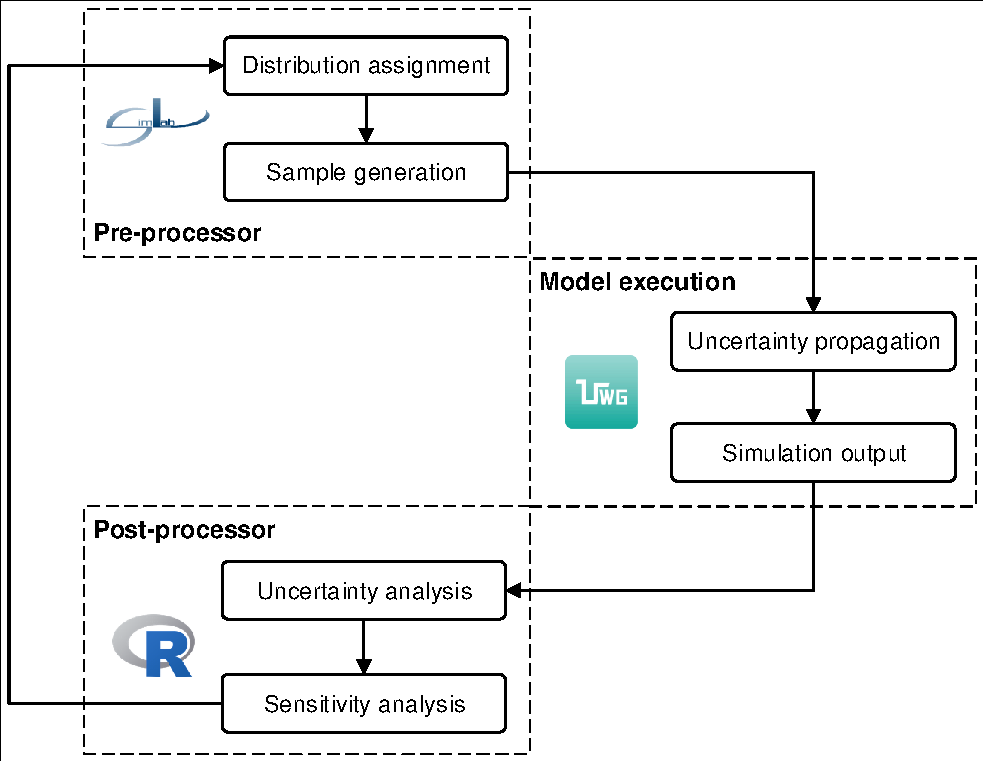
\includegraphics[width=.55\linewidth,trim=2 2 2 2,clip]{Framework.pdf}
\caption{General process of a global regression-based analysis using the \textsc{SimLab}, UWG, and \textsc{R} program.}
\end{figure}

The general analysis process is structured as shown in \textbf{Figure 4-3}. It starts by defining the distributions for aleatory and epistemic uncertainty and by producing the input samples automated via \textsc{SimLab}. Then, the sample data is read to create UWG input files via the Excel interface facilitated by \textsc{Matlab}. In the meantime, the \textsc{Matlab} code checks whether any severe or fatal errors occur during the parametric simulations. Finally, the outputs are collected to quantify the uncertainty/sensitivity indices, which is supported by the \textsc{R} sensitivity package. In the present study, effects due to the correlation between various inputs are assumed to be negligible.

The number of parametric simulations (sample size) for a reliable Monte Carlo analysis should be large enough to ensure convergence of the sensitivity indices but not be so large as to delay the SA process. For the regression-based analysis, although nearly no formal explanation has been presented, Saltelli et al. \cite{saltelli2004sensitivity} recommended the sample size of 1.5 -- 10 times the number of input parameters. Some researchers \cite{nguyen2015performance,menberg2016sensitivity} examined the convergence behavior with various simulation runs but gave quite different conclusions about the appropriate value. From the available experience and references, we choose to execute 1000 simulation runs for the summer and winter cases, respectively. This choice is a compromise between analysis accuracy and computational cost.

\subsection{Sensitivity index}

To estimate the sensitivity indices using the regression-based method, the model response is approximated by a multidimensional polynomial equation with a regression coefficient for each input. Then, the estimated regression coefficients are standardized using the variance of the corresponding input parameter and the variance of the model response \cite{saltelli2004sensitivity}. If a first-order polynomial is chosen, we will obtain the so-called standardized regression coefficient (SRC). The absolute value of the SRC represents a measure of parameter importance, with higher SRCs indicating more impact on the model output. In addition, the sign of the SRC shows whether the model output will increase or decrease as the corresponding input changes.

Many researchers \cite{tian2013review} have applied the sensitivity indices based on the rank transformation (SRRC) to investigate non-linear but monotonic models. However, the rank transformation techniques would change the model during the calculation, thereby leading to the sensitivity information of a different model \cite{saltelli2004sensitivity}. Such transformation would make the convergence of the sensitivity indices more difficult \cite{nguyen2015performance} and result in unstable outcomes. In addition, the available references indicate that the SRRC did not exhibit any outstanding performance \cite{de2009identification,nguyen2015performance}, while the SRC could keep quite stable and in good agreement with the indices from more sophisticated global SA methods \cite{menberg2016sensitivity}. Thus, the SRC is used in the present study to interpret a quantitative measure for the influence of the inputs on the model outputs.

However, the feasibility of the SRC is limited to the model responses that can be sufficiently approximated by the fitted regression model. The SRC is not reliable when the model under investigation is highly non-linear. In order to measure how well the regression model fits the model output, we use the coefficient of determination (R$^2$). Ranging from zero to one, the coefficient of determination tests how much the variance of the model response is explained by the variance of the regression model. The larger the R$^2$ is, the better the model will fit the data. Saltelli et al. \cite{saltelli2004sensitivity} have recommended a threshold of R$^2$ = 0.7 for a fairly strong regression model and its resulting SRCs.

\section{Model calibration}
 After the global SA is performed, the non-influential parameters will be fixed at some nominal values while the influential parameters will be further refined automatically via search and optimization algorithms. In particular, the Monte Carlo filtering technique and online hyper-heuristic evolutionary algorithm are proposed and developed in the present study. 

\subsection{Objective function}

Goodness-of-fit (GOF) is an index that relates the dispersion between the measured and simulated data via a statistical model. Many researchers \cite{ruiz2017analysis,reddy2007calibrating} have recommended and adopted the GOF as the objective for model calibration. Lower values mean that the model is more accurate and its behavior fits better with the real case. The GOF is defined as:

\begin{equation}
\textrm{GOF} = \sqrt{\frac{w^2_{\textrm{NMBE}} \textrm{NMBE}^2 + w^2_{\textrm{CV(RMSE)}} \textrm{CV(RMSE)}^2}{w^2_{\textrm{NMBE}} + w^2_{\textrm{CV(RMSE)}}}}\,,
\end{equation}
\vspace{12pt}
\noindent where
\vspace{0em}
\begin{equation}
\textrm{NMBE} = \frac{1}{\bar{m}} \frac{\sum_{i=1}^n (s_i - m_i)}{n}\,,
\end{equation}

\begin{equation}
\textrm{CV(RMSE)} = \frac{1}{\bar{m}} \sqrt{\frac{\sum_{i=1}^n (s_i - m_i)^2}{n-1}}\,.
\end{equation}

\vspace{15pt}
The NMBE (normalized mean bias error) quantifies the relative error of the simulated values with respect to the measured values summed over the selected number of time steps. Positive values indicate that the model over-estimates the actual scenarios, while the under-prediction produces negative values. As a counterpart, the CV(RMSE) (coefficient of variation of the root-mean-square error) indicates the variability of the errors (i.e., uncertainty) between the simulated ($s_i$) and measured ($m_i$) data. For numerical stability during optimization, $\bar{m}$ is set as the mean of the absolute values.

If the simulation results are plotted on an $x$-$y$ plane with NMBE and CV(RMSE) as the axes, one would like to identify a set of trade-off optimal solutions (i.e., a Pareto set) as the ``better'' solution set. This method is referred to as ``multi-objective optimization'' or ``Pareto optimization.'' For any given problem, the Pareto optimal set can be produced by an infinite number of Pareto points. A potential drawback of this approach is slower algorithm convergence and hence lower computational efficiency, compared with the performance of single-objective optimization \cite{ruiz2017analysis}. In addition, the problem of how to select the best solution from the Pareto set is not trivial since it depends on many aspects \cite{nguyen2014review}.

To avoid multi-objective optimization in the present case study, we use the idea of ``scalarization.'' Different weights are assigned to each index, and then the multi-objective function will be simplified as a weighted function of the criteria. Accordingly, we introduce a set of weights, $w_{\textrm{NMBE}}$ and $w_{\textrm{CV(RMSE)}}$, to impact our consolidated indices in Equation (4.1), where $w_{\textrm{NMBE}} + w_{\textrm{CV(RMSE)}} = 1$. Thus, the estimation of a Pareto front can be achieved by running single-objective optimizations with various weights.

In practice, energy and environment researchers would prefer the model to capture the bias (i.e., NMBE) more precisely than the variation (i.e., CV(RMSE)). This argument has been supported by the ASHRAE Guideline 14-2002 (RP-1051) \cite{reddy2007calibrating,guideline2002guideline}, which recommends a ratio of 3: 1 for $w_{\textrm{NMBE}}$: $w_{\textrm{CV(RMSE)}}$. Therefore, in the present study, we adopt this rule and set the $w_{\textrm{NMBE}}$ and $w_{\textrm{CV(RMSE)}}$ to be 0.75 and 0.25, respectively.

\subsection{Monte Carlo filtering}

Before conducting a fine calibration, it is important to reduce the dimensionality of the parameter space by identifying strong and weak parameters among the set of candidate inputs. Another intent is to detect the local ranges most likely to contain the ``actual'' value for each parameter. This can be achieved by adopting a blind Monte Carlo (MC) search coupled with sensitivity analysis (SA). In general, MC filtering is a process of rejecting sets of model outputs that are far from reality, while the SA can produce an influential parameter set that meets some prescribed criteria. Once the strong parameters are determined, the weak parameters can be fixed at some nominal values.

We have illustrated the details of regression-based SA through MC sampling in \textbf{Subsection 4.3}. After an LHMC batch run and regression-based analysis are completed, the strong parameters can be identified and the GOF indices can be computed for each trial. Those input vectors that result in unfavorable GOF values will be ruled out. On the other hand, the information contained in the ``good'' input vectors can be used to set values for the weak parameters, which can then be removed from further consideration in the calibration process. In particular, we use the average values of these promising input vectors to fix the weak parameters.

Once the MC filtering has identified a set of strong parameters, we can use the information advantageously to further fine-tune these influential inputs via heuristic-based search methods such as the evolutionary algorithm.

\subsection{Online hyper-heuristic evolutionary algorithm}

Evolutionary algorithms (EAs) have been widely used in a variety of complex real-world applications. However, EAs need to perform a large number of fitness (or objective) function evaluations in order to get optimal or near-optimal solutions. For engineering problems, each fitness function is evaluated via physics-based simulation, which often makes the whole process computationally expensive. Hyper-heuristics represent a class of methods that could address this barrier and reduce computational cost.

A hyper-heuristic search method seeks to automate, often by incorporation of statistical or machine learning techniques, the process of handling several simpler heuristics to efficiently solve computational search problems. The overall goal is to reduce the number of numerical simulations along a search path at the algorithm level. One popular paradigm is to construct a so-called surrogate or meta-model that can approximate the behavior of the original fitness function in the optimization process. The idea of hyper-heuristics can be traced back to the 1960s \cite{dunham1963design}, while managing approximate models in optimization via EAs has received continuous attention since the 1990s \cite{jin2005comprehensive}.

Based on how the surrogate models are used during the evolution, the hyper-heuristics can be further classified as \textit{offline} and \textit{online}. Offline hyper-heuristics utilize a surrogate model that is trained in advance, separately from the evolution process. This needs to be pre-validated and the surrogate must be updated to support a new case study. In online hyper-heuristics, a surrogate model is continuously retrained during the evolution and thus can make use of the most recent data. The self-updating mechanism without any pre-simulated database enables the online method to flexibly allow for many ``plug-and-play'' applications. Therefore, online hyper-heuristics have been very popular in engineering optimization problems \cite{tenne2010computational}.

\begin{table}[h]
\footnotesize
\begin{center}
\caption{Hyper-parameters of the evolutionary algorithm and support vector regression used in the model calibration.}
\label{my-label}
\begin{tabular}{ll}
\toprule
Hyper-parameter                         & Setting                        \\ \hline
\rule{0pt}{4ex}\textit{Evolutionary algorithm}\vspace{6pt}         &                                \\
\hspace{9pt}Algorithm type                          & Evolutionary strategy          \\
\hspace{9pt}Objective function                      & Goodness-of-fit                \\
\hspace{9pt}Parent population size $|P|$              & 120                            \\
\hspace{9pt}Offspring population size $|Q|$           & 120                            \\
\hspace{9pt}Surrogate population size $|S|$           & 360                            \\
\hspace{9pt}Maximum number of generations           & 60                             \\
\hspace{9pt}Maximum number of expensive evaluations & 2040                           \\
\hspace{9pt}Crossover algorithm                     & Laplace                        \\
\hspace{9pt}Crossover probability                   & 0.8                            \\
\hspace{9pt}Mutation algorithm                      & Power                          \\
\hspace{9pt}Mutation probability                    & 0.005                          \\
\hspace{9pt}Proportion of elitism                   & 0.2       \vspace{6pt}                    \\
\textit{Support vector regression}\vspace{6pt}      &                                \\
\hspace{9pt}Regression type                         & $\epsilon$-SV regression                \\
\hspace{9pt}Kernel function                         & Gaussian radial basis function \\
\hspace{9pt}Optimization method                     & Grid search                    \\
\hspace{9pt}Cross-validation                        & 5 folds                       
 \\
\bottomrule
\end{tabular}
\end{center}
Note: The hyper-parameters are set based on the prevailing engineering practices, previous related studies \cite{jin2005comprehensive,tenne2010computational,brownlee2015constrained,jin2011surrogate,deep2009real}, and trial and error. In particular, the surrogate population size is set to be three times of the parent population size \cite{brownlee2015constrained}, while the parent population size is set to be 10 times of the number of design parameters for single-objective optimization \cite{deep2009real}. The settings for the crossover and mutation operator follow the suggestions in Ref. \cite{deep2009real}. 
\end{table}

Although many researchers have utilized offline hyper-heuristics to calibrate the building energy models \cite{o2013leveraging,manfren2013calibration}, little is known to the author about the use of online hyper-heuristics. Very recently, some studies have been published to develop the online hyper-heuristic EAs for simulation-based multi-objective optimization in building design \cite{brownlee2015constrained,xu2016improving}. Therefore, we opt to embrace the methodology proposed by Brownlee and Wright \cite{brownlee2015constrained} and develop an online hyper-heuristic EA to calibrate an urban microclimate model. There are many possible ways to implement the general idea of online hyper-heuristics. The aim of this thesis is not to explore this whole space but simply to illustrate that one fairly straightforward application works well and that online surrogate model helps. As an illustrative example, the evolutionary strategy (ES) \cite{hansen1996adapting} in the \textsc{Matlab} environment and the support vector regression (SVR) \cite{cortes1995support} from LIBSVM \cite{chang2011libsvm} are selected for the present study due to their wide applications. \textbf{Table 4.2} summarizes the associated hyper-parameters. Although the convergence behavior of EA could be significantly affected by the hyper-parameters \cite{alajmi2014selecting}, we do not intend to explore this topic here and merely adopt some common settings.

\begin{figure}[h]
\centering
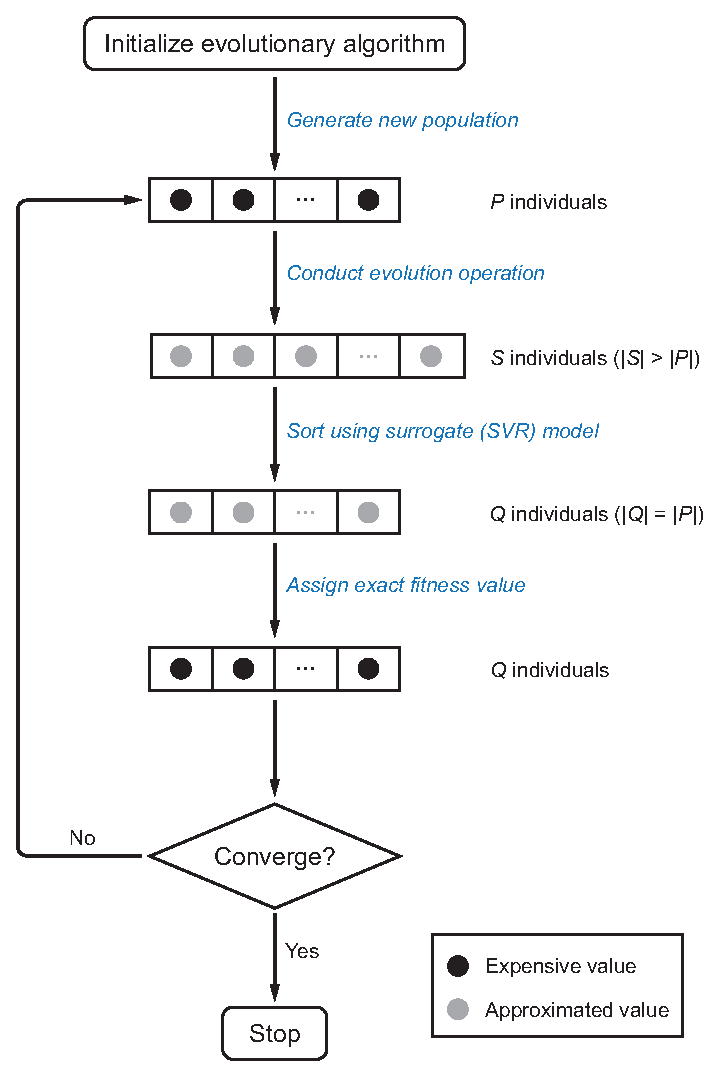
\includegraphics[width=.485\linewidth]{Figure4-3.eps}
\caption{General flowchart of an online hyper-heuristic EA (mainly from Ref. \cite{jin2011surrogate}).}
\end{figure}

\textbf{Figure 4-4} shows the procedure of an individual-based model management strategy, as described in Ref. \cite{jin2011surrogate}. In each generation, a local surrogate (SVR) model is trained if necessary. The role of SVR is to approximately evaluate the offspring in each generation and identify the most promising individuals among them, which will then be evaluated via expensive simulation. The latter are, of course, recorded and can be exploited as training patterns in the forthcoming generations. It is important to note that the surrogate model is \textit{not} used directly to examine the convergence behavior.

The pseudo-code of the proposed online hyper-heuristic EA for single-objective optimization is shown in \textbf{Algorithm 1}. The blue part (Steps 5-14) illustrates where and how a local surrogate model is built within the EA. At generation $t$, a surrogate (SVR) model needs to be updated if its accuracy is not acceptable. The SVR model is trained using the database $D$ that consists of previous population(s) $P$ and their expensive evaluations $F_{E,P}$ (Steps 5-10). Then, the crossover and mutation operators are used to generate a surrogate population $S$ (with size $|S| > |P|$) (Step 11). The SVR approximates the objective values in $S$ (Step 12), and the ES ranks $S$ (Step 13) with the highest ranking solutions inserted into the offspring population $Q$ (with size $|Q| = |P|$) (Step 14). $Q$ are then evaluated using the expensive UWG simulations, which will be appended into the database $D$ if they are not in $D$ before. Finally, the offspring $Q$ are assigned to be the parent $P$ in the next generation.

\begin{algorithm}[t]
\footnotesize
\caption{\textsc{Online Hyper-Heuristic Evolutionary Algorithm}}
\begin{algorithmic}[1]
\State initialize($P_t$) at $t$ = 1\Comment{Initialize new population}
\State $F_{E,P_t} = \textrm{obj-and-const-calc(} P_{t} \textrm{)}$\Comment{Expensive objective and constraint in $P$}
\State $D$ = cache($P_t$, $F_{E,P_t}$)\Comment{Store training data $P$ and $F$ into $D$}
\State \textbf{while} \textrm{not terminated} \textbf{do}
\color{blue}
\State \qquad \textbf{for all} \textrm{objective and constraint} \textbf{do}
\State \qquad\qquad \textrm{compute FPC in $P_{t}$}\Comment{Surrogate model performance}
\State \qquad\qquad \textbf{if} \textrm{FPC $<$ 0.7} \textbf{then}
\State \qquad\qquad \qquad \textrm{update-model($D$)}\Comment{Retrain model within the current generation}
\State \qquad\qquad \textbf{end if}
\State \qquad\textbf{end for}

\State \qquad $S = \textrm{make-new-pop(} P_{t} \textrm{)}$\Comment{Create surrogate population $S$ (with size $|S| > |P|$)}

\State \qquad $F_S = \textrm{obj-and-const-approx(} S \textrm{)}$\Comment{Approximated objective and constraint in $S$}

\State \qquad $S$ = rank($F_S, S$) \Comment{Rank individuals based on fitness values}

\State \qquad $Q_t$ = extract($S$) \Comment{Pre-select $Q$ individuals (with size $|Q| = |P|$)}
\color{black}

\State \qquad $F_{E,Q_t}$ = obj-and-const-calc($Q_t$) \Comment{Expensive objective and constraint in $Q$}

\State \qquad $D = D \cup (Q_t, F_{E,Q_t})$ \Comment{Add expensive evaluations into $D$}

\State \qquad $P_{t+1} = Q_t$ \Comment{Assign $Q$ as the next generation}

\State \qquad $t = t+1$\Comment{Increase generation counter}

\State \textbf{end while}

\end{algorithmic}
\end{algorithm}

The whole process continues until the evolution meets a stop criterion, e.g., the search exceeds the maximum number of generations or the maximum number of expensive simulations. In addition, we use a fitness prediction correlation (FPC) to measure the surrogate model accuracy. Usually the FPC is the Spearman's rank correlation, between the exact and approximated values, for one solution set. The threshold FPC for retraining is set as 0.7 \cite{brownlee2015constrained} for the present case study.